% !TEX root = main.tex

%%%%%%%%%%%%%%%%%%%%%%%%%%%%%%%%%%%%%%%%%%%%%%%%%%%%%%%%%%%%%%%%%%%%%%%%%%%%%%%%%%%%%%%%%%%%%%%%
\section{データ解析と考察}
%%%%%%%%%%%%%%%%%%%%%%%%%%%%%%%%%%%%%%%%%%%%%%%%%%%%%%%%%%%%%%%%%%%%%%%%%%%%%%%%%%%%%%%%%%%%%%%%

\begin{enumerate}
    \item 計算機実験の結果を第一週で得た電位𝑉の空間分布実験結果の上に上書きせよ.
    そして,それらを比較して,一致点と相違点を全て列挙せよ.
    \begin{description}
        \item[] 計算機実験の結果を第1週で得た電位$V$の空間分布実験結果の上に
        上書きしたものを図5に示す.
    \end{description}
    
    \begin{itemize}
        \item 一致点
        \begin{description}
            \item[] $y$座標が小さくなるほどが原点に引っ張られるような等電位線となっており,
            $x$座標が正において「く」の字型,$x$座標が負において,逆「く」の字型になっている.
        \end{description}

        \item 相違点
        \begin{description}
            \item[] $x$座標が正において,シミュレーション結果の方が高い電圧となっており,
            $x$座標が負の範囲において,シミュレーション結果の方が低い電圧となっている.
        \end{description}
    \end{itemize}

    \item 設問(1)における相違点が現れてきた理由を説明せよ.
    \begin{description}
        \item[] 第1週目の実験課題1において,電極板付近の電圧がは$6.0\,\si{\volt}$
        となっており,理論上の印加電圧である$10\,\si{\volt}$よりも低くなっている.
        $V=Ed$より,等電位面がずれ,相違点が現れたと考えられる.
    \end{description}
\end{enumerate}

\begin{figure}[H]
    \begin{center}
        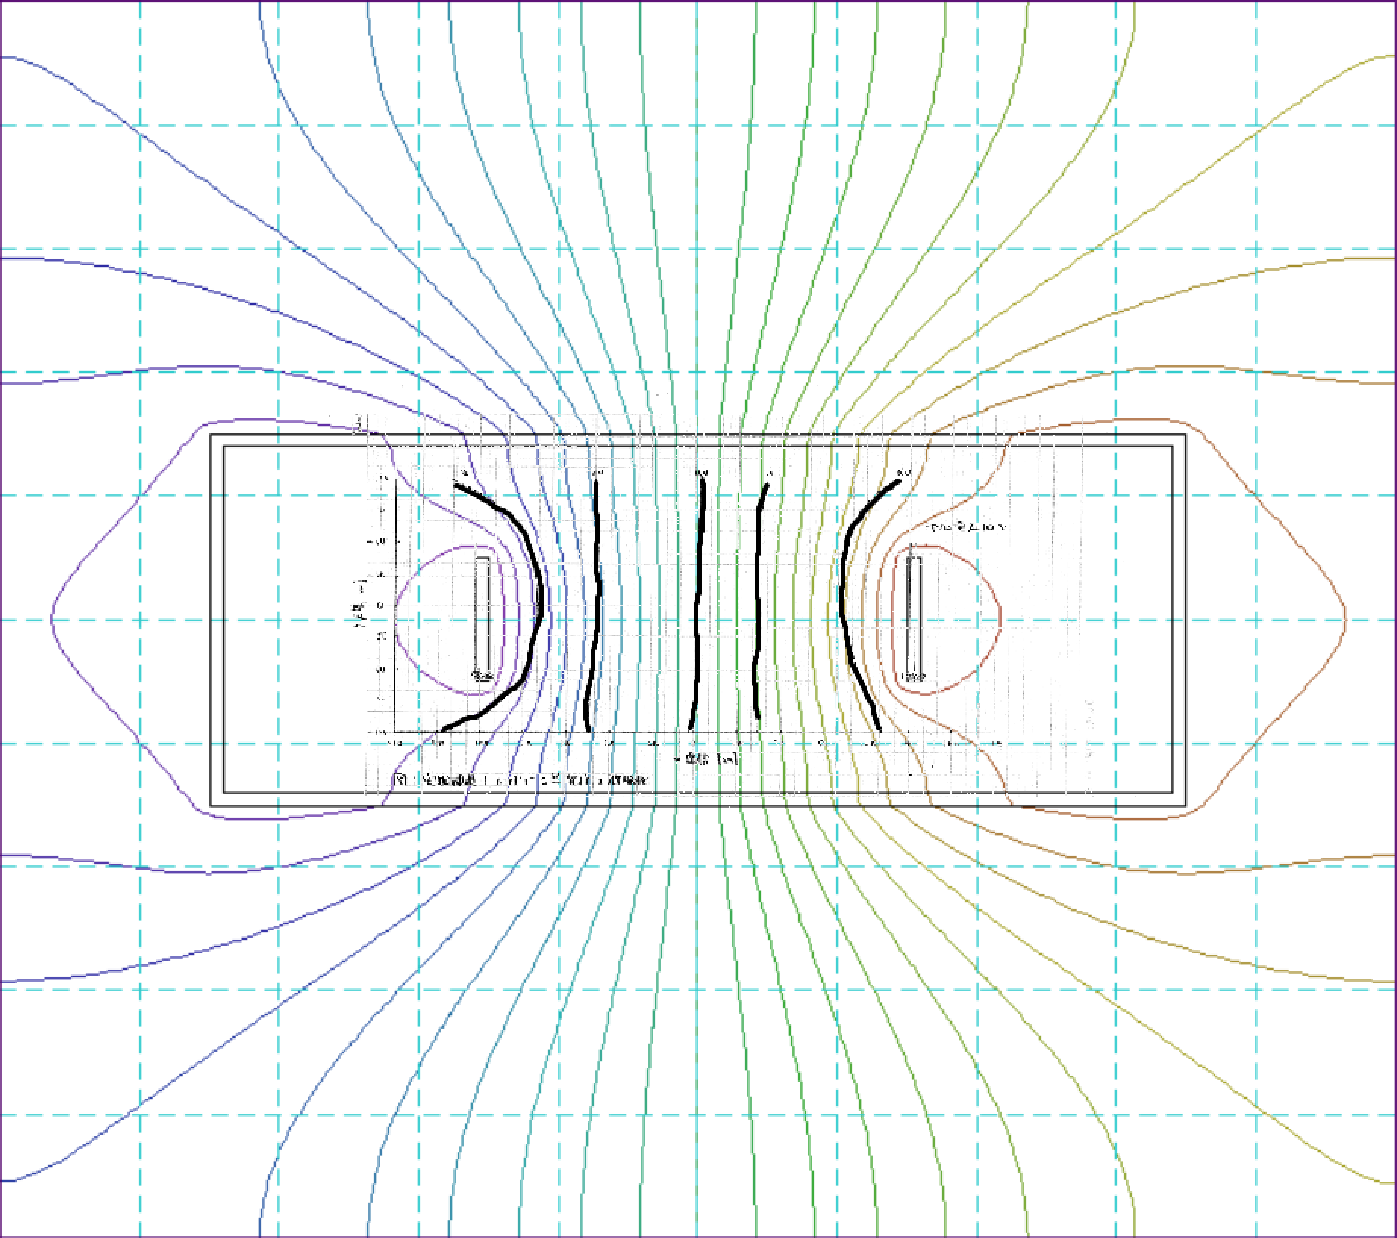
\includegraphics[scale=0.5]{figure5.pdf}
        \caption{計算機実験と第1回目の実験の空間分布の比較}
    \end{center}
\end{figure}